    \section{Présentation de Gittip}


\begin{frame}
\frametitle{Quelques chiffres\ldots}

\begin{itemize}
    \itemsep1.5em
    \item Système open source de micro-dons réguliers
    \item Dons hebdomadaires (chaque mardi)
    \item Créé le 11 mai 2012 par \textbf{Chad Whitacre}
    \item Novembre 2013 :
        \begin{itemize}
            \item \textbf{22 000} utilisateurs, dont \textbf{2 000} actifs.
            \item \textbf{7 300\euro{}} au total transférés chaque semaine
        \end{itemize}
\end{itemize}
\end{frame}


    \subsection{Un système de micro-dons libre}


{
\logo{}
\begin{frame}
\frametitle{Aspects communautaires}
\begin{center}
\begin{columns}
\begin{column}{280px}
{
    \begin{figure}[h!]
        \centering
        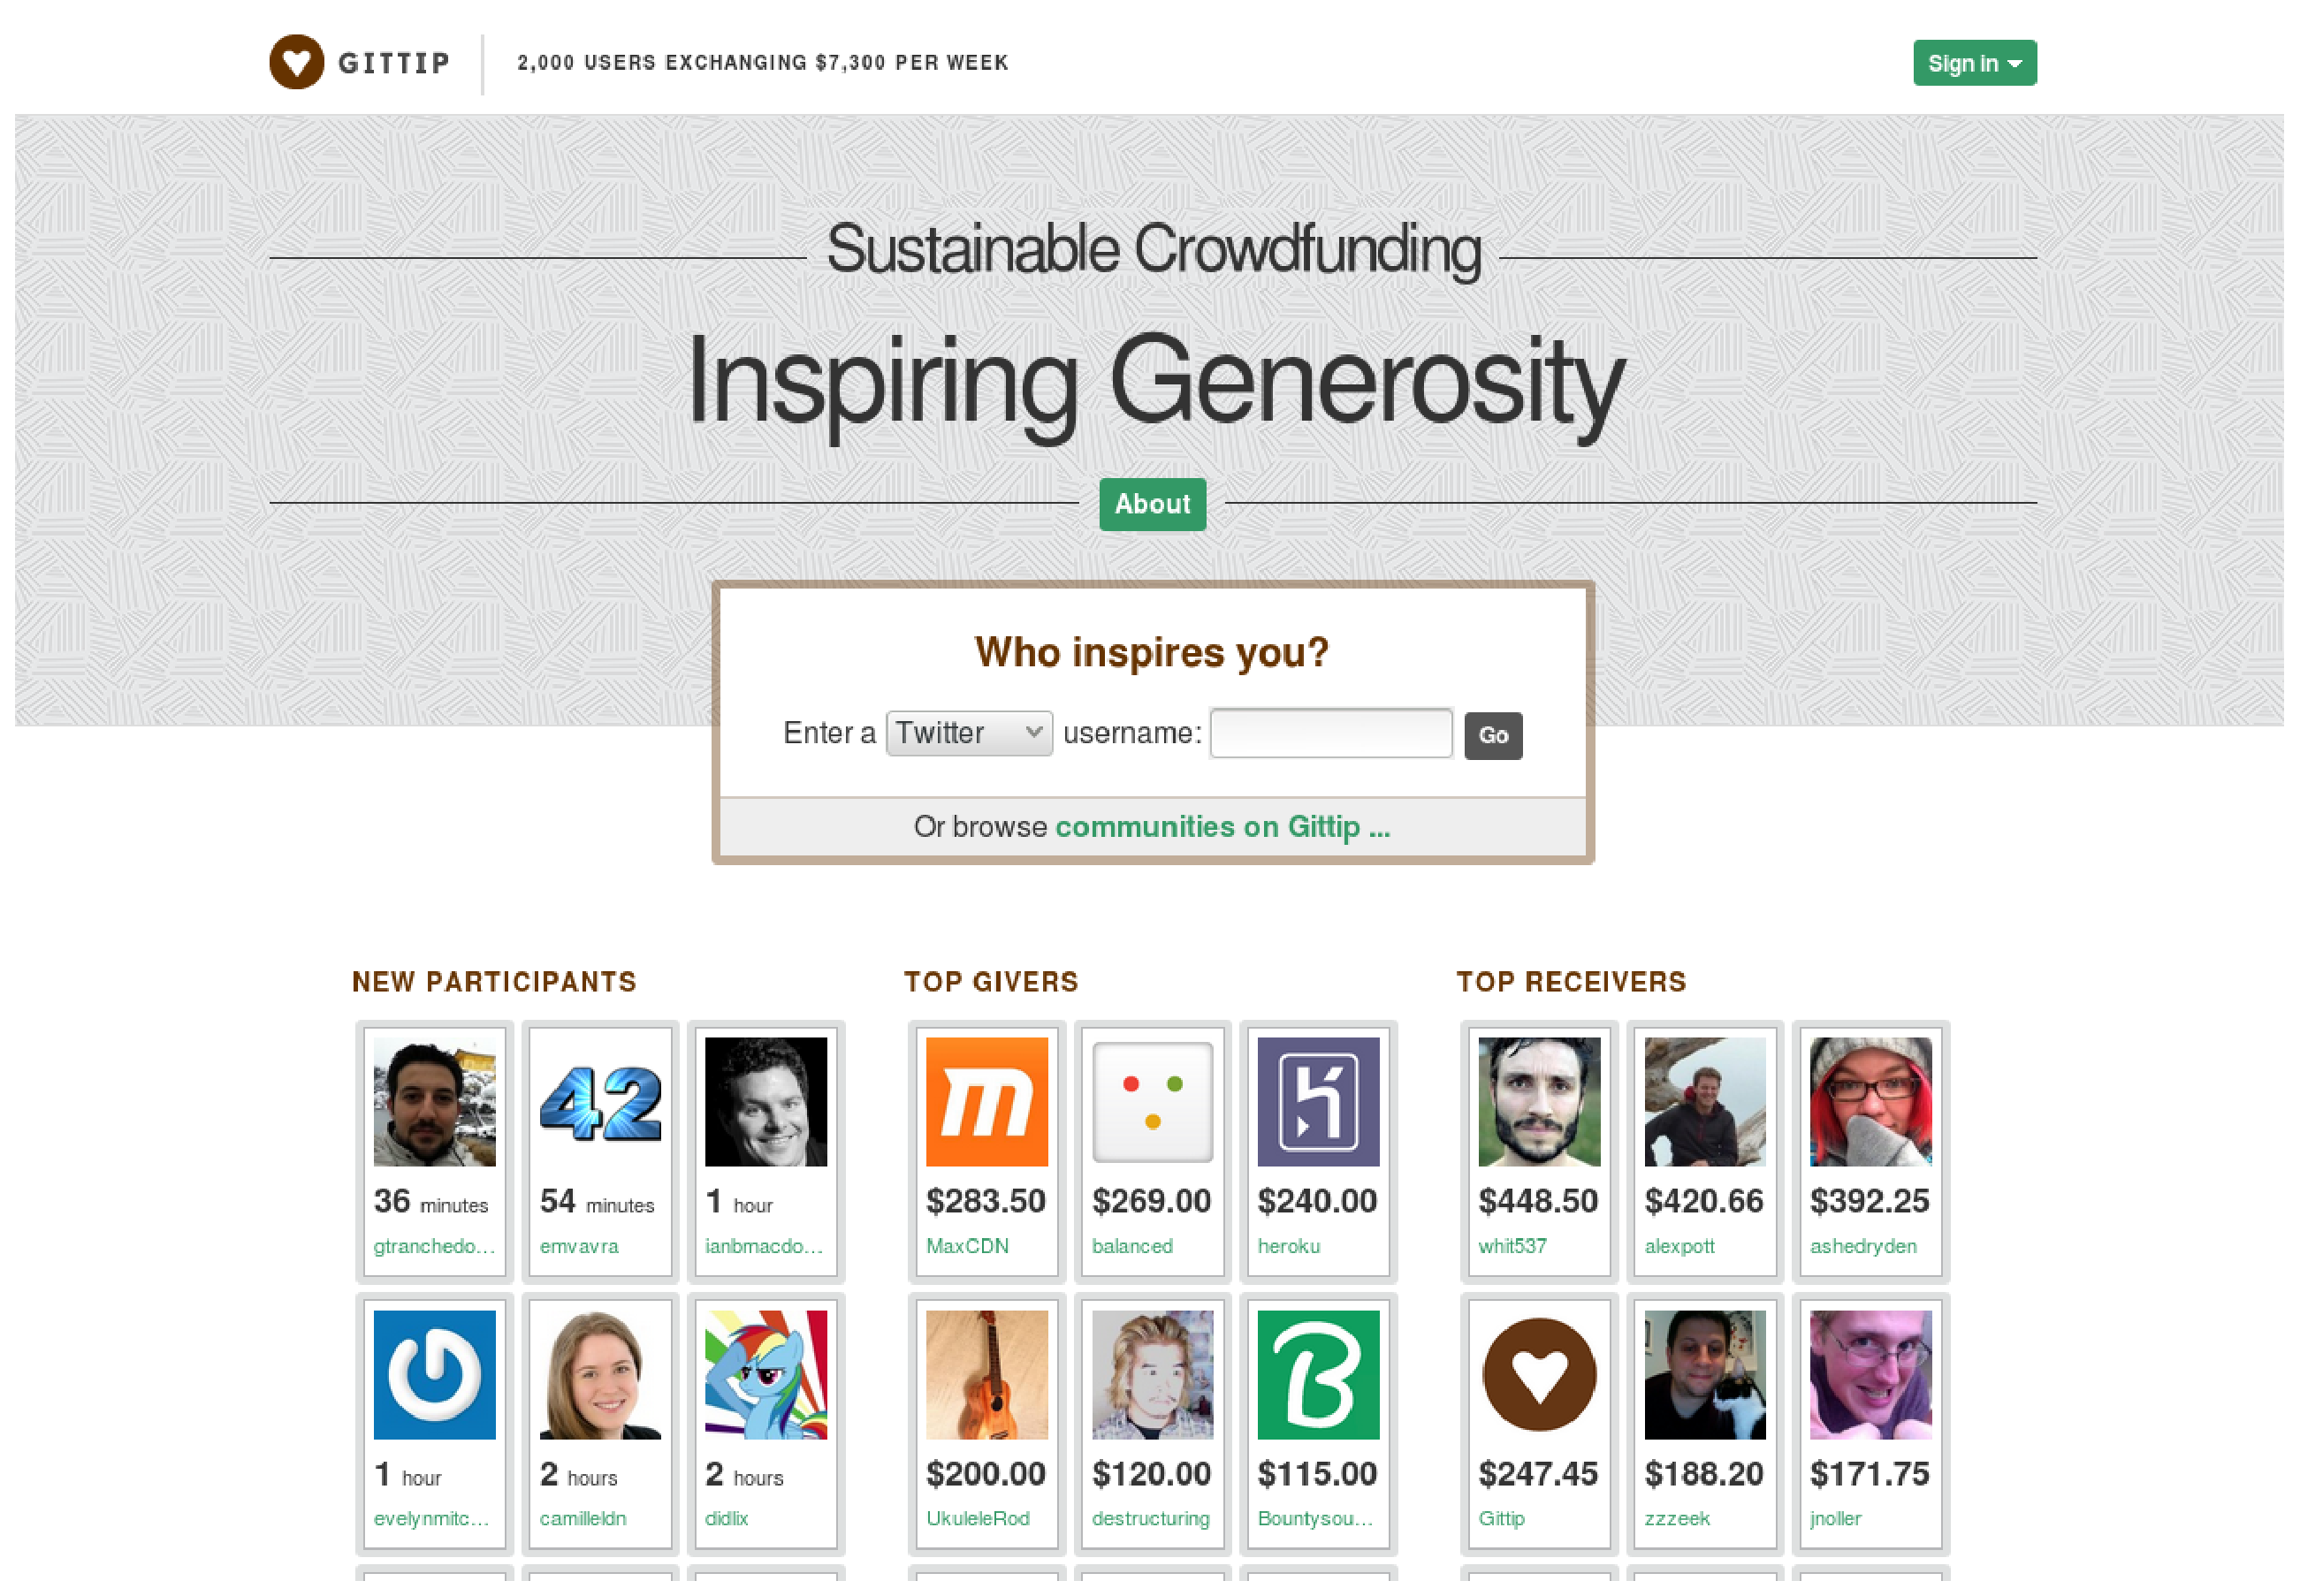
\includegraphics[width=260px]{images/section1/homepage-gittip.eps}
        \caption{Page d'accueil de gittip.com}
    \end{figure}
}
\end{column}
\end{columns}
\end{center}
\end{frame}
}


{
\logo{}
\begin{frame}
\begin{center}
\begin{columns}
\begin{column}{280px}
{
    \begin{figure}[h!]
        \centering
        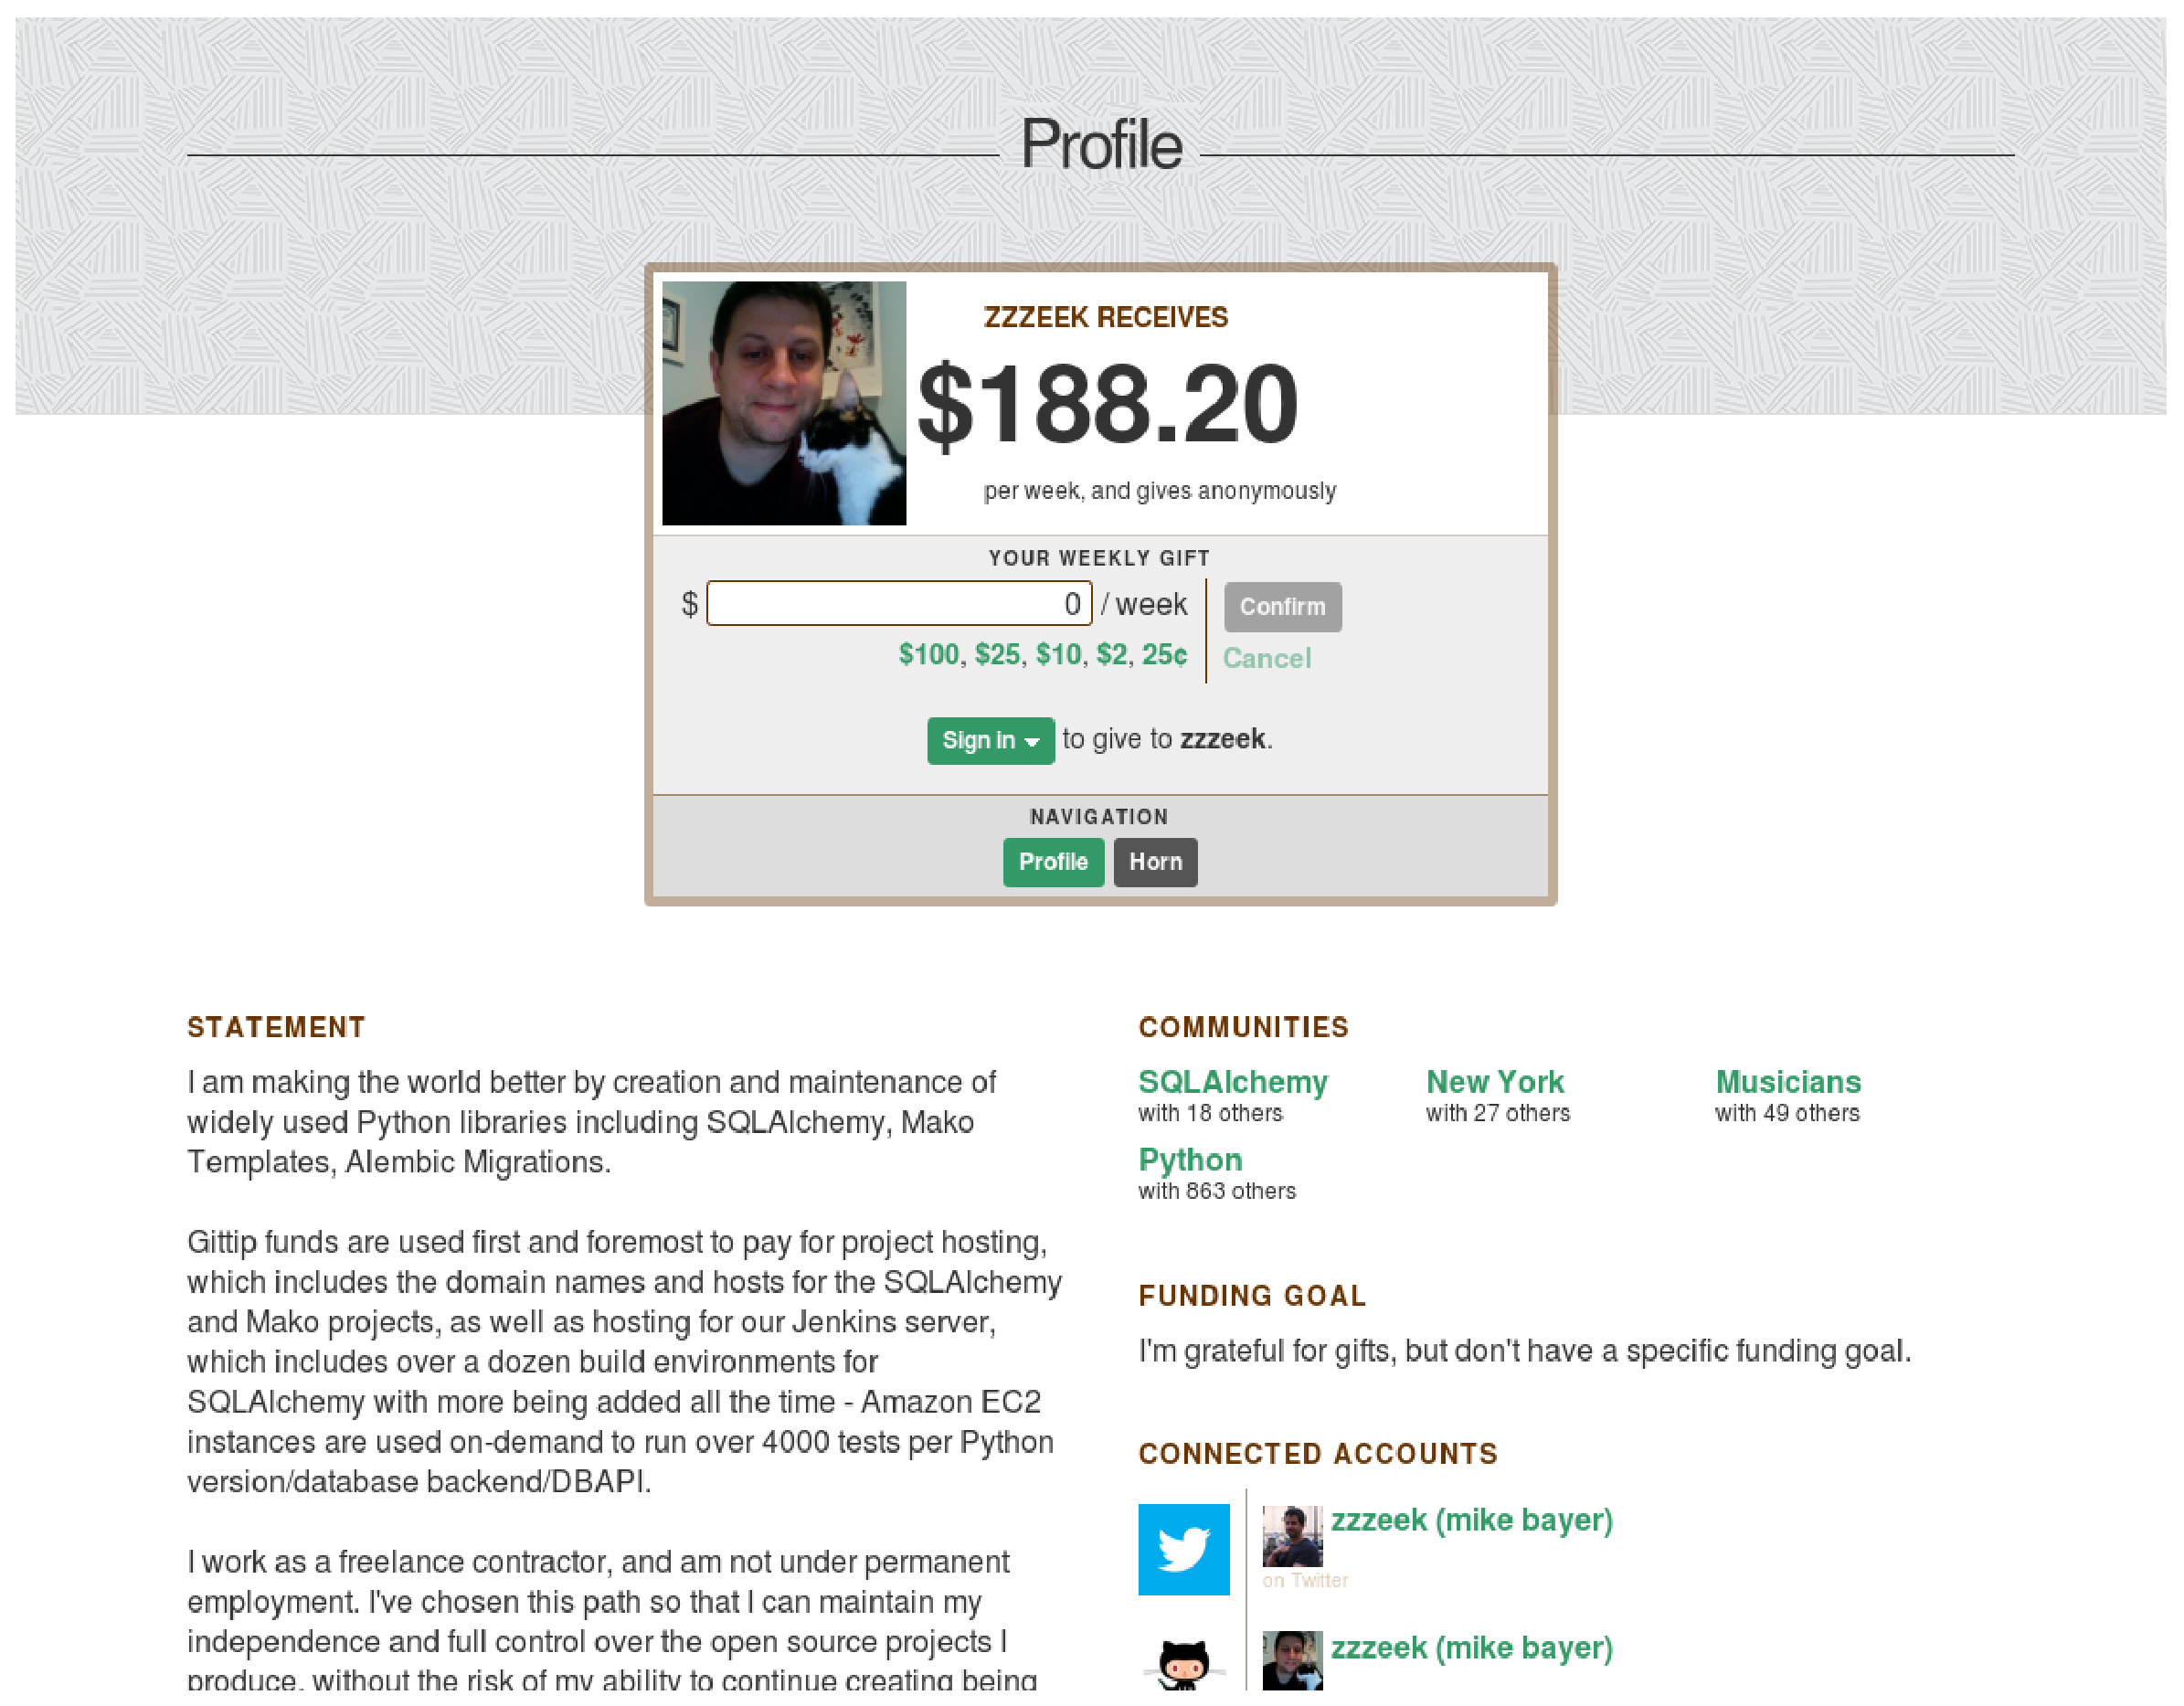
\includegraphics[width=260px]{images/section1/profilepage-gittip.eps}
        \caption{Exemple d'une page de profil sur gittip.com}
    \end{figure}
}
\end{column}
\end{columns}
\end{center}
\end{frame}
}


    \subsection{L'open company Gittip LLC}


\begin{frame}
\frametitle{L'open company \emph{Gittip LLC}}

\begin{itemize}
    \itemsep1.5em
    \item Créée en février 2012 par Chad Whitacre
    \item 2ème open company
    \item Basée sur la transparence
    \item Sans hiérarchie
\end{itemize}
\end{frame}
